\documentclass[a4paper]{article}

%% Language and font encodings
\usepackage[english]{babel}
\usepackage[utf8x]{inputenc}
\usepackage[T1]{fontenc}

%% Sets page size and margins
\usepackage[a4paper,top=3cm,bottom=2cm,left=3cm,right=3cm,marginparwidth=1.75cm]{geometry}

%% Useful packages
\usepackage{amsmath}
\usepackage{graphicx}
\usepackage[colorinlistoftodos]{todonotes}
\usepackage[colorlinks=true, allcolors=blue]{hyperref}

\title{Reporte de Actividad 3\\ Sondeos meteorológicos de la Atmósfera}
\author{Michelle Contreras Cossio}
\date{14 de Febrero del 2018}

\begin{document}
\maketitle

\section{Introducción}

En el presente trabajo se muestran los resultados de la Actividad 3 de Física Computacional, donde se utilizaron datos, proporcionados por la Universidad de Wyoming, sobre sondeos atmosféricos; la zona de la cual se recogieron los datos fue el Aeropuerto Internacional de la ciudad de Adelaida, ubicada en Australia Meridional. Además se recogieron datos únicamente del 22 de Diciembre y del 22 de Junio del 2017, solsticios de invierno y verano respectivamente. \\

Estos datos se trataron, con Python, para crear gráficas que nos permitan comparar como cambia la atmósfera en el día más largo y más corto del año. Los pasos llevados acabo durante el procesamiento de estos datos, así como los resultados obtenidos se presentan en este documento. 

\section{Fundamentos}
La atmósfera terrestre es una capa que rodea a nuestro planeta, compuesta de gases, coloquialmente conocida como "aire". Esta compuesta principalmente de nitrógeno, oxígeno, argón, dióxido de carbono, vapor de agua y otros gases. \\

La densidad y presión disminuyen a mayor altitud en la atmósfera, sin embargo, la temperatura no tiene un patrón continuo. Este hecho permite distinguir entre las diferentes capas que conforman a la atmosfera, dándose una estratificación en cinco capas principales que son, desde la parte superior hasta la inferior: 
\begin{itemize}
\item Exosfera: 700 a 10,000 km 
\item Termosfera: 80 a 700 km 
\item Mesosfera: 50 a 80 km
\item Estratosfera: 12 a 50 km 
\item Troposfera: 0 a 12 km 
\end{itemize} 

Los datos utilizados recaban información únicamente de la Troposfera y Estratosfera, las dos capas inferiores, dentro de las cuales se ubica la capa de ozono y donde ocurren la mayoría de los fenómenos meteorológicos. Sin embargo, en la Troposfera, la temperatura decrece con la altitud, hasta la tropopausa; por otro lado, en la Estratosfera, la temperatura aumenta con la altitud. 

\section {Análisis de Datos}

Como fue mencionado con anterioridad, primeramente se tomaron los datos, de la base de datos de sondeos atmosféricos por la Universidad de Wyoming, en la locación escogida, que fue el Aeropuerto Internacional de la ciudad de Adelaida, en Australia; de los días 22 de Diciembre y 22 de Junio, ambos del 2017. Estos se descargaron del sitio web proporcionado y se guardaron dos archivos txt bajo el nombre de 22dic y 22jun.

Para poder crear las gráficas (presentadas en la sección de resultados), se debieron trabajar estos datos, utilizando jupyter, con las bibliotecas de pandas, Numpy y PyPlot. Primeramente, se leyendo ambos archivos asignandolos, cada uno, a una variable correspondiente, saltando los renglones innecesarios; se procedió a crear un nuevo data frame para cada uno de los dos conjuntos de datos, con la particularidad de que se omitieran los renglones que no aportaban datos, así como los últimos (27) renglones con información inutilizada para estos fines.

\begin{figure}[h!]
  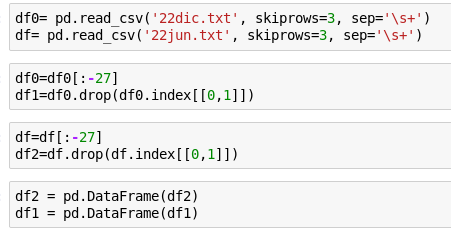
\includegraphics[width=10cm]{1.png}
  \centering
  \label{fig:1}
\end{figure}

Y a manera de verificación de que los datos estan completos y sin información que no corresponde a los datos a estudiar, se imprimieron el encabezado y pie de cada data frame creado. 
\begin{figure}[h!]
  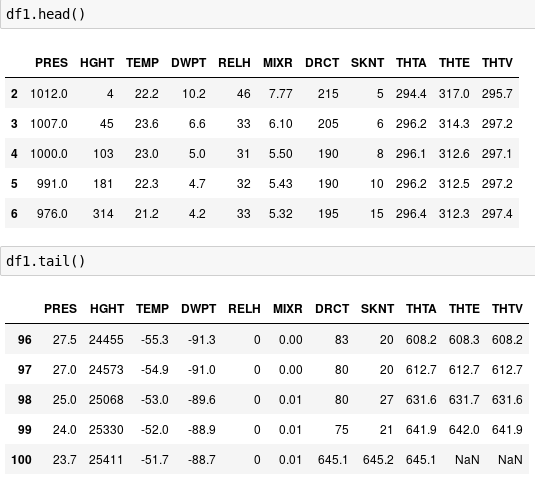
\includegraphics[width=7cm]{2.png}
  \centering
  \label{fig:2}
\end{figure}
\begin{figure}[h!]
  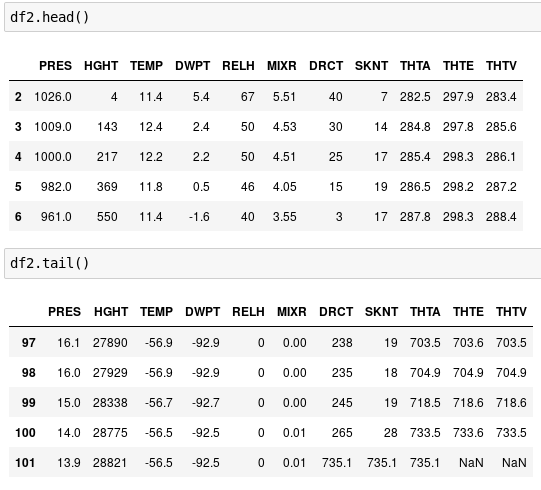
\includegraphics[width=7cm]{3.png}
  \centering
  \label{fig:3}
\end{figure}

Debido a que se leyeron unos datos no numéricos, que posteriormente se omitieron, pandas clasificó a todos los datos como objetos, sin embargo, se utilizó una función que nos permitió convertir las columnas con las que trabajamos, a datos numéricos: 

\begin{figure}[h!]
  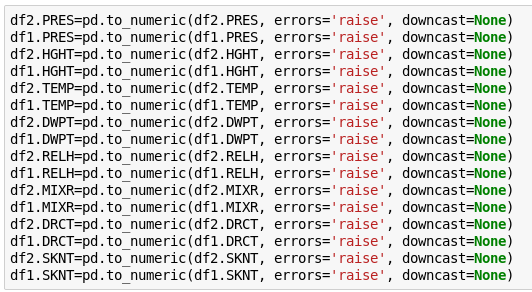
\includegraphics[width=7cm]{4.png}
  \centering
  \label{fig:4}
\end{figure}

Así, nuestros datos fueron convertidos a numéricos y se pudo exitosamente trabajar con ellos para el desarrollo de las gráficas requeridas por la actividad. 

\section {Resultados}

A continuación se presentan las gráficas realizadas durante la actividad de los dos días solicitados. \\

\textbf{Gráficas de Altitud vs Presión:}

\begin{figure}[h!]
  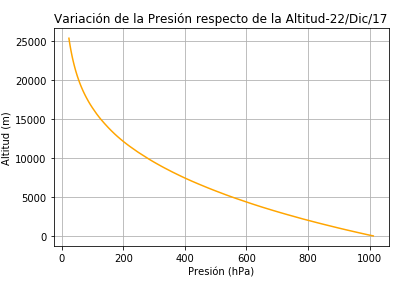
\includegraphics[width=10cm]{graf1.png}
  \centering
  \label{fig:5}
\end{figure}

\begin{figure}[h!]
  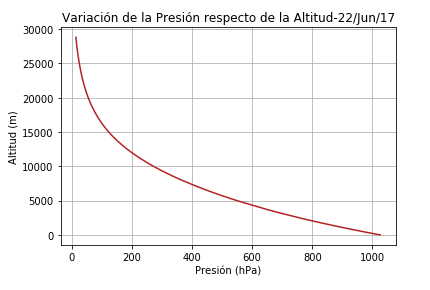
\includegraphics[width=10cm]{graf2.png}
  \centering
  \label{fig:6}
\end{figure}

Con estas gráficas, podemos notar que la Altura es inversamente proporcional a la Presión, aunque no sobre un factor lineal, mas bien exponencial.

\newpage
\textbf{Gráficas de Altitud vs Temperatura:}

\begin{figure}[h!]
  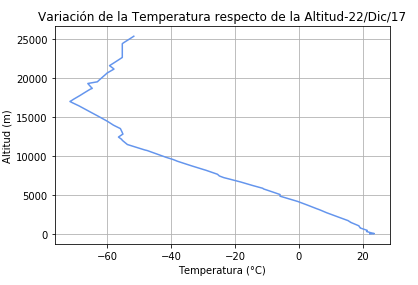
\includegraphics[width=10cm]{graf3.png}
  \centering
  \label{fig:7}
\end{figure}

\begin{figure}[h!]
  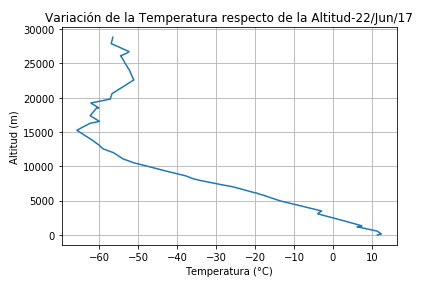
\includegraphics[width=10cm]{graf4.png}
  \centering
  \label{fig:8}
\end{figure}

¿Hay cambios significativos en la tropopausa entre las dos fechas? Como fue mencionado durante la sección de fundamentos, la Tropopausa marca el punto o "pico" donde la temperatura deja de descender con la altitud y empieza a ascender. El cambio, aunque no es tan visual, por la escala, es de aproximadamente 2.5 km. El 22 de diciembre, la tropopausa se ubica aproximadamente a los 17.5 km de altitud, mientras que el 22 de junio, se ubica a los 15km. \\

\textbf{Gráficas de Altitud vs Temperatura y Temperatura de rocío:}

\begin{figure}[h!]
  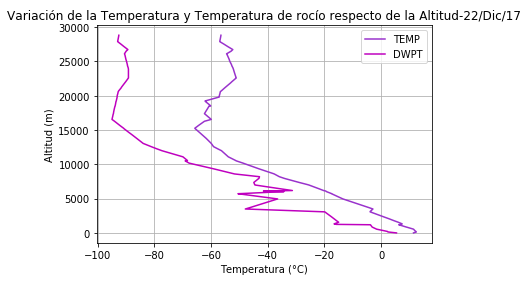
\includegraphics[width=10cm]{graf5.png}
  \centering
  \label{fig:9}
\end{figure}

\begin{figure}[h!]
  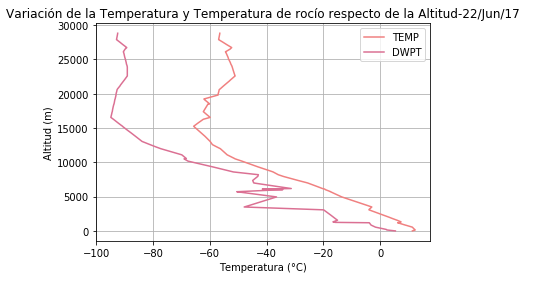
\includegraphics[width=10cm]{graf6.png}
  \centering
  \label{fig:10}
\end{figure}

La temperatura y temperatura de rocío se comportan de manera similar, disminuyen hasta llegar a la tropopausa y de ahí empuezan a aumentar.\\

\textbf{Gráficas de la rapidez de los vientos:}

\begin{figure}[h!]
  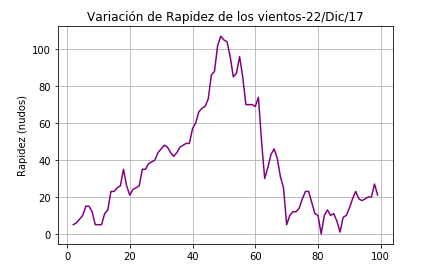
\includegraphics[width=10cm]{graf7.png}
  \centering
  \label{fig:11}
\end{figure}

\begin{figure}[h!]
  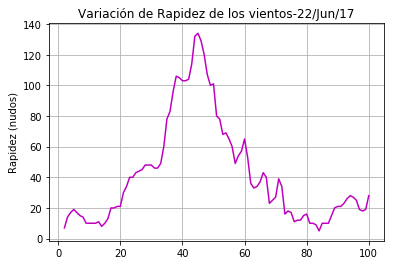
\includegraphics[width=10cm]{graf8.png}
  \centering
  \label{fig:12}
\end{figure}

Ambas gráficas tienen un comportamiento similar, la rapidez va en subida, llega a un pico, mas o menos a la mitad del día, y después desciende.

\newpage
\textbf{Gráficas de la Humedad Relativa como función de la Altura:}

\begin{figure}[h!]
  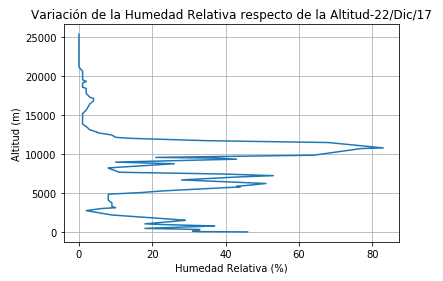
\includegraphics[width=10cm]{graf9.png}
  \centering
  \label{fig:13}
\end{figure}

\begin{figure}[h!]
  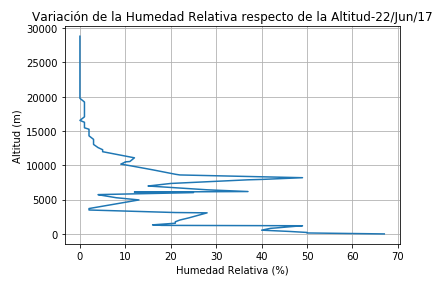
\includegraphics[width=10cm]{graf10.png}
  \centering
  \label{fig:14}
\end{figure}

Con estas gráficas no fue posible observar un patrón que nos indique como es la variación de la humedad con respecto a la altura, sin embargo, lo que si puede notarse es que después de la tropopausa, en ambos casos, no existe gran variación. 

\section {Conclusión}

Con esta actividad se puede concluir que en ocasiones el análisis de los datos es una parte fundamental para poder trabajar con los mismos, es decir, que la parte de graficar es sencilla, en comparación a la limpieza y estética de datos, que implica mayor detenimiento y observación en que estos datos hayan sido leídos justo como lo queremos. \\

Una vez teniendo los datos en orden, la parte de graficar se vuelve más fácil, ya que prácticamente es siempre lo mismo, mientras que cada archivo de datos es diferente y necesita diferente formato.\\

Otra cosa que me gustaría agregar es que fue completamente necesario poner atención a cada detalle o problema que podrían tener los datos, ya que, por ejemplo, cuando no aceptaba los datos como numéricos, no permitía graficar, así pues, con esta experiencia, aprendí que no debemos tomar por hecho que python va a entender todo sin antes configurarlo. 

\section{Bibliografía}

\begin{itemize}
\item Atmospheric Soundings. (2018). Consultado: 8 de Febrero del 2018, de University of Wyoming, Department of Atmospheric Science. Sitio web:  \\
http://weather.uwyo.edu/upperair/sounding.html
\item Atmosphere of Earth.(2018). Consultado: 13 de Febrero del 2018, de Wikipedia. Sitio web: \\
https:$//$en.wikipedia.org$/$wiki$/$Atmosphere\_of\_Earth
\item Estratosfera.(2018). Consultado: 13 de Febrero del 2018, de Wikipedia. Sitio web: \\
https://es.wikipedia.org/wiki/Estratosfera 
\item Termosphere.(2018). Consultado: 13 de Febrero del 2018, de Wikipedia. Sitio web: \\
https://en.wikipedia.org/wiki/Thermosphere
\end{itemize}


\section{Apéndice}
\begin{enumerate}
\item ¿Cuál es tu opinión general de esta actividad?

Me gustó, cada vez se me hace más sencillo el manejo de Python y sobre todo al momento de graficas, me permitió encontrarle más sentido.

\item ¿Qué fue lo que más te agradó? ¿Lo que menos te agradó?

Poder identificar las diferentes formas de graficar y realmente entenderlo. Lo que menos me agradó fue encontrarme con que no me leía los datos como numéricos, pero es un problema que pude enfrentar y sacar adelante.

\item ¿Que consideras que aprendiste en esta actividad? 

Aprendí como puedo automatizar una mejor captura de datos, cada vez más eficiente y pulí un poco mi conocimiento en gráficas.

\item ¿Qué le faltó? ¿O le sobró?  

Siento que estuvo bien el contenido, ni mucho, ni poco, suficiente para poder digerirlo con calma.

\item ¿Que mejoras sugieres a la actividad?

Ninguna. 

\end{enumerate}

%
\end{document}